% Created 2021-10-30 Sat 00:09
% Intended LaTeX compiler: pdflatex
\documentclass[10pt, xcolor=svgnames]{beamer}
\usepackage[utf8]{inputenc}
\usepackage[T1]{fontenc}
\usepackage{graphicx}
\usepackage{grffile}
\usepackage{longtable}
\usepackage{wrapfig}
\usepackage{rotating}
\usepackage[normalem]{ulem}
\usepackage{amsmath}
\usepackage{textcomp}
\usepackage{amssymb}
\usepackage{capt-of}
\usepackage{hyperref}
\usepackage{tikz}
\usetikzlibrary{calc}
\usetikzlibrary{arrows} % For nice arrow tips (Align-BDD)
\setbeamertemplate{blocks}[rounded][shadow=false]
\usepackage{bibentry}
\nobibliography*
% This file determines notation
% and defines various helper commands.
% (loaded after all packages)

% some common notation
% \newcommand{\defeq}{\stackrel{\text{def}}{=}} % and my heart is broken as I
% comment this out... :(
\newcommand{\defeq}{=}

% Notation specific to Align-BDD project
\renewcommand{\vec}[1]{\mathbf{#1}} % just bold vectors, no arrows
\newcommand{\sn}[0]{\textbf{Step  \arabic{ALG@line}.}}
\newcommand{\swap}[0]{\texttt{swap}}
\newcommand{\sift}[0]{\texttt{sift}}
\newcommand{\Ninst}[0]{$10,048$}
\newcommand{\PVAL}[0]{0.6}

% some code needed for algorithms description (appendix) >>>
\newcommand{\CL}{\texttt{current-layer}}
\newcommand{\NL}{\texttt{next-layer}}
\newcommand{\IFN}{\texttt{infeasible-node}}
\newcommand{\add}[3]{\textbf{add node} to $D$: #1
  $\overset{\textrm{#2}}\longrightarrow$ \textit{(new)} #3}
\newcommand{\link}[3]{\textbf{add arc} to $D$: #1
  $\overset{\textrm{#3}}\longrightarrow$ #2 }
\newcommand{\state}{\texttt{state}}
\newcommand{\crit}{\texttt{critical-nodes}}
\newcommand{\nstate}{\texttt{next-state}}
\newcommand{\cov}{\texttt{C}}
\newcommand{\type}{\texttt{T}}
\newcommand{\hi}[1]{\texttt{HI(#1)}}
\newcommand{\lo}[1]{\texttt{LO(#1)}}

\newcommand{\F}{\textbf{F}}
\newcommand{\T}{\textbf{T}}
\newcommand{\HI}{\texttt{HI}}
\newcommand{\LO}{\texttt{LO}}
\newcommand{\ROOT}{\texttt{r}}
\newcommand{\N}{\mathcal{N}}
\newcommand{\var}{\textrm{var}}
\newcommand{\true}{\texttt{True}}
\newcommand{\false}{\texttt{False}}
\newcommand{\BN}{\mathbb{B}^N}
\newcommand{\X}{\mathbb{X}^N}
\newcommand{\orig}{\ref{probl:ap}$(A,B;T^*)$}
\newcommand{\simpl}{\ref{probl:ap}$(S_A,S_B;T_\VS^*)$}
\newcommand{\SN}{\mathbb{S}^N}
\newcommand{\VS}{\textrm{VS}}
\newcommand{\erem}{\hfill \Halmos}    % ends a remark or an example
\newcommand{\vv}{\vec{v}}

% \algdef{SE}[SUBALG]{Indent}{EndIndent}{}{\algorithmicend\ }%
% \algtext*{Indent}
% \algtext*{EndIndent}

% One style for all TikZ pictures for working with overlays:
% \tikzset{every picture/.style=remember picture}
% % Define a TikZ node for math content:
% \newcommand{\mathnode}[2]{%
%   \mathord{\tikz[baseline=(#2.base), inner sep = 0pt]{\node (#2) {$#1$};}}}

% Notation specific to DSPI algorithms notation
\newcommand{\ahat}{\widehat{\alpha}}
\newcommand{\bhat}{\widehat{\beta}}

\newcommand{\rnode}{\texttt{root}}
\newcommand{\argmin}{\textrm{argmin}}
\newcommand{\argmax}{\textrm{argmax}}
\newcommand{\und}{\textrm{ and }}
\newcommand{\isnot}[1]{\textrm{ is not }\textit{#1}} %{\not\sim\textrm{ ``#1''}}
\newcommand{\is}[1]{\sim\textrm{ ``#1''}}
\newcommand{\mrk}[1]{\texttt{mark}(#1)}

% # tree / algo specific notation
\newcommand{\actions}[1]{\texttt{actions}(#1)}
\newcommand{\children}[1]{\texttt{children}(#1)}
\newcommand{\pos}[1]{\textrm{p}(#1)}
\newcommand{\FS}[1]{\textrm{FS}(#1)}

\makeatletter
\def\LB{\@ifstar\@LB\@@LB}
\def\@LB{\textit{LB}}
\def\@@LB#1{\textit{LB}(#1)}

\def\UB{\@ifstar\@UB\@@UB}
\def\@UB{\textit{UB}}
\def\@@UB#1{\textit{UB}(#1)}
\makeatother

\newcommand{\newnode}[1]{\textrm{\textbf{create node}(#1)}}

% Horizontal algo phase section separation
\newcommand{\panelsep}{\vspace{0.7em} {\color{lightgray}\hrule} \vspace{0.7em}}
\newcommand{\psep}{\vspace{0.5em}}
\usetheme{Darmstadt}
\author{Alexey Bochkarev}
\date{2021-11-02, 08-30, Zoom / Freeman Hall 123}
\title{Selected Topics in Network Optimization: Aligning BDDs for a Facility Location Problem and a Search Tree Method for DSPI.}
\subtitle{Dissertation defense}
\hypersetup{
 pdfauthor={Alexey Bochkarev},
 pdftitle={Selected Topics in Network Optimization: Aligning BDDs for a Facility Location Problem and a Search Tree Method for DSPI.},
 pdfkeywords={},
 pdfsubject={},
 pdfcreator={Emacs 28.0.50 (Org mode 9.4.5)}, 
 pdflang={English}}
\begin{document}

\maketitle
\begin{frame}{Outline}
\tableofcontents
\end{frame}


\section{{\bfseries\sffamily TODO} Aligning BDDs}
\label{sec:orgda14710}
\subsection{On BDD representations}
\label{sec:org39a7528}
\subsection{BDD alignment (``original'') problem}
\label{sec:org32d4f59}
\subsection{The simplified problem}
\label{sec:org2b3a4ed}
\subsection{Numerical experiments}
\label{sec:org27b5420}

\section{{\bfseries\sffamily TODO} A BDD-based approach to a Facility Location Problem}
\label{sec:org04ea660}
\subsection{Problem description}
\label{sec:orge4528b2}
\subsection{BDD representation}
\label{sec:org21b2383}
\subsection{Solving the CPP}
\label{sec:orgcf4bcbf}
\subsection{Numerical experiments}
\label{sec:org5a08bbc}

\section{Monte Carlo Tree Search for DSPI}
\label{sec:org7700361}
\subsection{Problem formulation}
\label{sec:orgbed14e0}
\begin{frame}[label={sec:orgf3a62b1}]{A game of ``interdiction'': intro}
\begin{columns}
\begin{column}[t]{0.4\columnwidth}
\begin{center}
\includegraphics[width=.9\linewidth]{./img/SPI.png}
\end{center}
\end{column}

\begin{column}[t]{0.6\columnwidth}
\begin{itemize}
\item \alert{Network:} a directed graph with two special nodes (source \textcircled{s} and terminal \textcircled{t}), and a pair of "costs" associated to each edge.
\item \alert{User:} seeks to run through the graph, \textcircled{s} to \textcircled{t}, at min cost.
\item \alert{Attacker:} maximizes the User's cost by "attacking" the arcs, having a limited "budget".
\end{itemize}

We consider a \alert{dynamic} version of the game, following \cite{sefair2016}. (NP-hard)
\end{column}
\end{columns}
\end{frame}

\begin{frame}[label={sec:orgd43ba44}]{A game of ``interdiction'': formulation}
The Interdictor's optimal objective \(z^*\) can be expressed as:
\begin{equation*}
z^*(S,i) = \max_{S^\prime \subseteq \FS{i}\setminus S~:~|S\cup S^\prime|\leq b} \Big\{\min_{j\in\FS{i}} \{z^*(S\cup S^\prime, j) + \widetilde{c}_{ij}(S\cup S^\prime)\}\Big\},
\end{equation*}
where:
\begin{itemize}
\item \(S\): interdiction set,
\item \(i\): current Evader's node, \(\FS{i}\) -- forward star of node \(i\),
\item \(\widetilde{c}_{ij}\): arc traversal costs (given the interdiction),
\item \(b\): Interdictor's budget.
\end{itemize}
\pause

\begin{block}{Existing algorithms (by Sefair \& Smith)}
\begin{itemize}
\item polynomial DP algorithm for a DAG
\item exact DP algorithm, exp time for general case.
\end{itemize}
\end{block}
\end{frame}

\subsection{What do we propose?}
\label{sec:org842b7e9}
\begin{frame}[label={sec:orga094104}]{Monte Carlo Tree Search}
\begin{itemize}
\item Maintain the game tree,
\item Try not to create all the nodes,
\item Prune the definitely suboptimal ones,
\item Drive the tree growth by a computationally cheap objective estimate (e.g.,
based on simulated games).
\end{itemize}
\end{frame}

\subsection{MCTS framework}
\label{sec:orgf956fa4}
\begin{frame}[label={sec:orgac17577}]{The ``game tree''}
Create a ``game tree'', where \alert{nodes} contain the following information.
\begin{itemize}
\item Current \alert{status}
\begin{itemize}
\item \(\pos{j}\in \mathcal{N}\): where is the Evader,
\item \(S_j\subseteq \mathcal{A}\): what is interdicted,
\item \(\tau(j)\): who's turn is it (Interdictor/Evader)\pause
\end{itemize}
\item Possible further \alert{development}
\begin{itemize}
\item \(\children{j}\): child game tree nodes,
\item \(\actions{j}\): available actions.\pause
\end{itemize}
\item \alert{Costs} info, to drive the search and prune the tree
\begin{itemize}
\item \(\widehat{Q}_j\): cost-to-go (starting from this node),
\item \(\LB{j},~\UB{j}\): bounds on the true cost-to-go,
\item \(N_j\in\mathbb{N}\): how many times the node was visited\pause
\end{itemize}

So, we iterate through \alert{episodes}, each one implying a ``full cycle'' of the game tree update in four \alert{phases}.
\end{itemize}
\end{frame}

\tikzstyle{sel} = [minimum size=2mm, NavyBlue]
\tikzstyle{stdnode} = [draw, fill, circle, lightgray, minimum size=2mm]
\tikzstyle{empty} = [draw=none, fill=none]
\tikzstyle{rootnode} = [fill=none]
\tikzstyle{edge from parent} = [draw=lightgray]

\begin{frame}[label={sec:org3f8cc5d}]{Phase 1. Selection}
\begin{minipage}{0.3\textwidth}
% selection
\begin{tikzpicture}[%level distance=5mm,
level 1/.style={level distance=10mm,sibling distance=12mm},
level 2/.style={level distance=10mm,sibling distance=7mm},
level 3/.style={level distance=10mm,sibling distance=7mm},
font=\scriptsize,inner sep=2pt,every node/.style=stdnode]

\node[NavyBlue, sel] {} % root
child {node {}
        child {node {}} 
        child {node {} 
            child {node{}} 
            child {node{}}
        }
    edge from parent }
child {node {}}
child   {[NavyBlue] node[sel] {}
            child {[black] node {}}
            child {node[sel] {}
                   edge from parent[NavyBlue]
            }
        edge from parent[NavyBlue]
        };
\end{tikzpicture}
\end{minipage}\hfill
\begin{minipage}{0.5\textwidth}
\textbf{What's happening:}
\begin{itemize}
  \item Start at the root node,
  \item Use \textit{tree policy} to choose the next node recursively...
  \item ... pruning nodes as we go, when possible ...
  \item ... until we reach a leaf.
\end{itemize}
\psep{}

\textbf{What's updated:}
\begin{itemize}
  \item Nothing in the tree.
  \item Along the way: bounds for pruning (more momentarily!) + path costs.
\end{itemize}
\end{minipage}
\end{frame}
\begin{frame}[label={sec:orgdd8e96e}]{Phase 2. Expansion}
% expansion
\begin{minipage}{0.3\textwidth}
\begin{tikzpicture}[%level distance=5mm,
level 1/.style={level distance=10mm,sibling distance=12mm},
level 2/.style={level distance=10mm,sibling distance=7mm},
level 3/.style={level distance=10mm,sibling distance=7mm},
font=\scriptsize,inner sep=2pt,every node/.style=stdnode]

\node[rootnode] {} % root
child {node {}
        child {node {}} 
        child {node {} 
            child {node{}} 
            child {node{}}
        }
    edge from parent }
child {node {}}
child   {node {}
            child {node {}}
            child {node {}
                child {[NavyBlue] node[sel]{} edge from parent[NavyBlue]}
                child {[NavyBlue] node[sel]{} edge from parent[NavyBlue]}
                child {[NavyBlue] node[sel]{} edge from parent[NavyBlue]}
            }
        };
\end{tikzpicture}
\end{minipage}\hfill
\begin{minipage}{0.5\textwidth}
\textbf{What's happening:}
\begin{itemize}
  \item Create child nodes for possible actions.
\end{itemize}
\psep{}

\textbf{What's updated:}
\begin{itemize}
  \item New nodes are created,
  \item UBs and LBs are calculated
\end{itemize}\psep{}

\textbf{Note:} Some inconsistencies can be introduced here, between child and parent nodes.
\end{minipage}
\end{frame}
\begin{frame}[label={sec:orga567d35}]{Phase 3. Roll-outs}
% roll-outs
\begin{minipage}{0.3\textwidth}
\begin{tikzpicture}[%level distance=5mm,
level 1/.style={level distance=10mm,sibling distance=12mm},
level 2/.style={level distance=10mm,sibling distance=7mm},
level 3/.style={level distance=10mm,sibling distance=7mm},
font=\scriptsize,inner sep=2pt,every node/.style=stdnode]

\node[rootnode] {} % root
child {node {}
        child {node {}} 
        child {node {} 
            child {node{}} 
            child {node{}}
        }
    edge from parent }
child {node {}}
child {node {}
       child {node {}}
       child {node {}
              child {node[sel] (a1) {}
                     child {node[empty, NavyBlue] (b1) {...} edge from parent[draw=none]
                       child{node[sel, fill=none] (c1) {}
                             edge from parent[draw=none]}}}
                child {node[sel] (a2) {}
                    child {node[empty, NavyBlue] (b2) {...} edge from parent[draw=none]
                       child{node[sel, fill=none] (c2) {}
                             edge from parent[draw=none]}}}
                child {node[sel] (a3) {}
                    child {node[empty, NavyBlue] (b3) {...} edge from parent[draw=none]
                       child{node[sel, fill=none] (c3) {}
                             edge from parent[draw=none]}}}}
                             };
\draw[bend left, NavyBlue, shorten <=2pt] (a1) to (b1);
\draw[->, bend right, NavyBlue, shorten >= 2pt] (b1) to (c1);
\draw[bend right, NavyBlue, shorten <=2pt] (a2) to (b2);
\draw[->, bend left, NavyBlue, shorten >=2pt] (b2) to (c2);
\draw[bend left, NavyBlue, shorten <=2pt] (a3) to (b3);
\draw[->, bend right, NavyBlue, shorten >=2pt] (b3) to (c3);
\draw[dashed, NavyBlue, rounded corners=7] ($(c1)+(-.3,.3)$)rectangle($(c3)+(.3,-.3)$);
\node[draw=none, fill=none, yshift=-4.5mm, NavyBlue] at ($(c1)!.5!(c3)$){Terminal nodes}; 
\end{tikzpicture}%
\vspace{-2.5em}
\end{minipage}\hfill
\begin{minipage}{0.5\textwidth}
\textbf{What's happening:}
\begin{itemize}
  \item Run a random simulated game from each node,
  \item Calculate cost-to-go estimate $\widehat{Q}_j$ as the simulated game cost.
\end{itemize} \psep{}

\textbf{What's updated}
\begin{itemize}
  \item Cost-to-go for each new node.
\end{itemize}\psep{}

\textbf{Note:} We do not record the intermediate game states occured during roll-outs!
\end{minipage}
\end{frame}

\begin{frame}[label={sec:org938aadd}]{Phase 4. Backpropagation}
% backpropagation
\begin{minipage}{0.3\textwidth}
\begin{tikzpicture}[%level distance=5mm,
level 1/.style={level distance=10mm,sibling distance=12mm},
level 2/.style={level distance=10mm,sibling distance=7mm},
level 3/.style={level distance=10mm,sibling distance=7mm},
font=\scriptsize,inner sep=2pt,every node/.style=stdnode]

\node[sel] (d) {} % root
child {node {}
        child {node {}} 
        child {node {} 
            child {node{}} 
            child {node{}}
        }
    edge from parent }
child {node {}}
child {node[sel] (c) {}
            child {node {}}
            child {node[sel] (b) {}
                child {node{}}
                child {node{}}
                child {node[sel] (a) {}}
            }
        };

\draw[->, NavyBlue, bend right, shorten >=2pt, shorten <=2pt] (a) to (b.east);
\draw[->, NavyBlue, bend right, shorten >=2pt, shorten <=2pt] (b.north east) to (c.east);
\draw[->, NavyBlue, bend right, shorten >=2pt, shorten <=2pt] (c.north east) to (d.east);
\end{tikzpicture}
\end{minipage}\hfill
\begin{minipage}{0.5\textwidth}
\textbf{What's happening:}
\begin{itemize}
  \item Start at the selected node,
  \item Recursively update (``propagate'') node information for parents ...
  \item ... until we reach the root.
\end{itemize} \psep{}

\textbf{What's updated:}
Information in each parent node, using the child nodes:
\begin{itemize}
  \item UBs and LBs
  \item Cost-to-go estimate: the best value (given the turn).
\end{itemize}
\end{minipage}
\end{frame}

\begin{frame}[label={sec:orgebb0aa0}]{The Algorithm}
The algorithm can perform actions for both players. Each turn involves two
steps:\vspace{2ex}

\begin{columns}
\begin{column}[t]{0.4\columnwidth}
\textbf{Step 1.} THINK.\vspace{1ex}

We iteratively improve the tree (while we have budget):\vspace{1ex}

\textbf{FOR} \(k=1,\ldots, K\) \textbf{DO}
\begin{itemize}
\item Selection
\item Expansion
\item Roll-outs
\item Backpropagation
\end{itemize}
\textbf{END.}
\end{column}

\begin{column}[t]{0.4\columnwidth}
\textbf{Step 2.} ACT.\vspace{1ex}

\ldots{} then pick an action corresponding to the ``most
attractive'' child node of the root.
\end{column}
\end{columns}
\end{frame}

\begin{frame}[label={sec:org42ae126}]{There are several secret ingredients}
\begin{figure}
\includegraphics[width=\textwidth]{img/ingredient.jpg}
\end{figure}
\end{frame}

\begin{frame}[label={sec:org96e4ac3}]{SI-1. How to select?}
\begin{itemize}
\item \textbf{with probability $\varepsilon$}: choose at random;
\item \textbf{otherwise}, a child node with the \alert{best score}:
\end{itemize}
\begin{equation*}
R_j \defeq \underbrace{\sigma_i (\widetilde{C}_{ij} + \widehat{Q}_j)}_{\textrm{best cost-to-go}} ~~+ ~~\underbrace{C_p\sqrt{\log(N_i) / N_j}}_{\textrm{encourage exploration}}, \quad \textrm{ for all } j\in\children{i}
\end{equation*}

``Best'' here depends on the turn (the Evader will choose the smallest cost estimate, the Interdictor --- the largest).
\end{frame}
\begin{frame}[label={sec:orgdf91dcc}]{SI-2. How to prune?}
We leverage the classic idea of \alert{alpha--beta pruning}:
\vspace{2ex}
\begin{columns}
\begin{column}{0.4\columnwidth}
\begin{tikzpicture}[%level distance=5mm,
level 1/.style={level distance=10mm,sibling distance=12mm},
level 2/.style={level distance=10mm,sibling distance=7mm},
level 3/.style={level distance=10mm,sibling distance=7mm},
font=\scriptsize,inner sep=2pt,
edge from parent/.style={draw=black},
every node/.style={draw, circle}]

\node[label=above:{root}]{I} % root
child {node[label=left:{$(A)$}] {E}
        child {node[label=below:{$j^{\prime\prime}$}] {I}} 
        child {node[sel, label=below:{$j^\prime$}] {I}} 
        child {node {I}} 
    edge from parent node[draw=none, left] {pass}}
child {node {I}}
child   {node[sel, label=right:{$(B)$}] {I}
            child {node {I}
                child {node[draw=none] {...}}
                child {node[draw=none] {...}}}
            child {node {I}
                child {node[draw=none] {...}}}
        edge from parent};
\end{tikzpicture}
\end{column}
\begin{column}{0.6\columnwidth}
Maintain two running numbers (bounds):
\begin{itemize}
\item \(\alpha\): the worst (minimum) alternative cost achievable by the Interdictor,
\item \(\beta\): the worst (maximum) alternative cost achievable by the Evader.
\end{itemize}
\vspace{2ex}
 \alert{Pruning condition:} \(\beta \leq \ahat_j\) or \(\bhat_j \leq \alpha\), where
\begin{itemize}
\item \(\ahat_j =\pi_n+\LB{j}\)  (Interdictor's turns), and
\item \(\bhat_j = \pi_n+\widetilde{C}_{nj} + \UB{j}\) (Evader's turns)
\end{itemize}
\end{column}
\end{columns}
\end{frame}
\begin{frame}[label={sec:org97287ac}]{SI-3. How to back-propagate?}
Assuming the Evader's turn, and \(i\) being the current game tree node:
\begin{itemize}
\item Update the bounds:
\end{itemize}
\begin{align*}
  \UB{i} &\gets \min_{j\in\children{i}} \Big\{ \widetilde{C}_{ij}(S_i) + \UB{j} \Big\},\\
  \LB{i} &\gets \min_{j\in\children{i}} \Big\{ \widetilde{C}_{ij}(S_i) + \LB{j} \Big\}.
\end{align*}

\begin{itemize}
\item Update the cost-to-go estimate:
\end{itemize}
\begin{equation*}
\widehat{Q}_i \gets \min_{j\in\children{i}} \Big\{ \widetilde{C}_{ij}(S_i) + \widehat{Q}_j\Big\}.
\end{equation*}
\end{frame}
\subsection{Numerical experiments}
\label{sec:org412346c}
\begin{frame}[label={sec:org6c9ee69}]{Numerical experiments: strategy}
\begin{itemize}
\item How does it perform on pre-defined instances? (relative to the known optimum, and to the bounds)
\item How does it perform on randomly generated instances with different budgets?
\item What's the dynamics of the tree construction? How does the algorithm work?
\item What's the point of ``playing out'', i.e., changing root nodes?
\end{itemize}
\end{frame}

\begin{frame}[label={sec:org9d415d5}]{Pre-defined instances}
\begin{figure}
\includegraphics[width=\textwidth]{img/fig_known.png}
\end{figure}
\end{frame}
\begin{frame}[label={sec:orgdfe1a00}]{Random instances (snapshot)}
\begin{figure}
\includegraphics[width=\textwidth]{img/fig_bounds.png}\vspace{0.5ex}
\includegraphics[width=\textwidth]{img/fig_runtimes.png}
\end{figure}
\end{frame}
\begin{frame}[label={sec:org2df8e1b}]{Convergence profiles}
\begin{minipage}{0.45\textwidth}
{\scriptsize \centering $\varepsilon=0.05$\vspace{1ex} \\}
\includegraphics[width=0.4\paperwidth]{img/conv_profile_2eps_0.05.png}
\end{minipage}\hfill
\begin{minipage}{0.45\textwidth}
{\scriptsize \centering $\varepsilon=0.5$\vspace{1ex} \\}
\includegraphics[width=0.4\paperwidth]{img/conv_profile_2eps_0.5.png}%
\end{minipage}
\end{frame}
\begin{frame}[label={sec:orgcf66d3a}]{A remark: that's not just different runs}
\begin{columns}
\begin{column}{0.6\columnwidth}
\includegraphics[height=0.8\textheight]{img/treesizes.png}
\end{column}
\begin{column}{0.4\columnwidth}
For each value of \(\varepsilon\) (0.05, 0.5, and 1) we performed three runs, to confirm these are indeed different ``modes'' of the algorithm.
\end{column}
\end{columns}
\end{frame}

\begin{frame}[label={sec:org189f3d5}]{Play-out vs. first-move strategy}
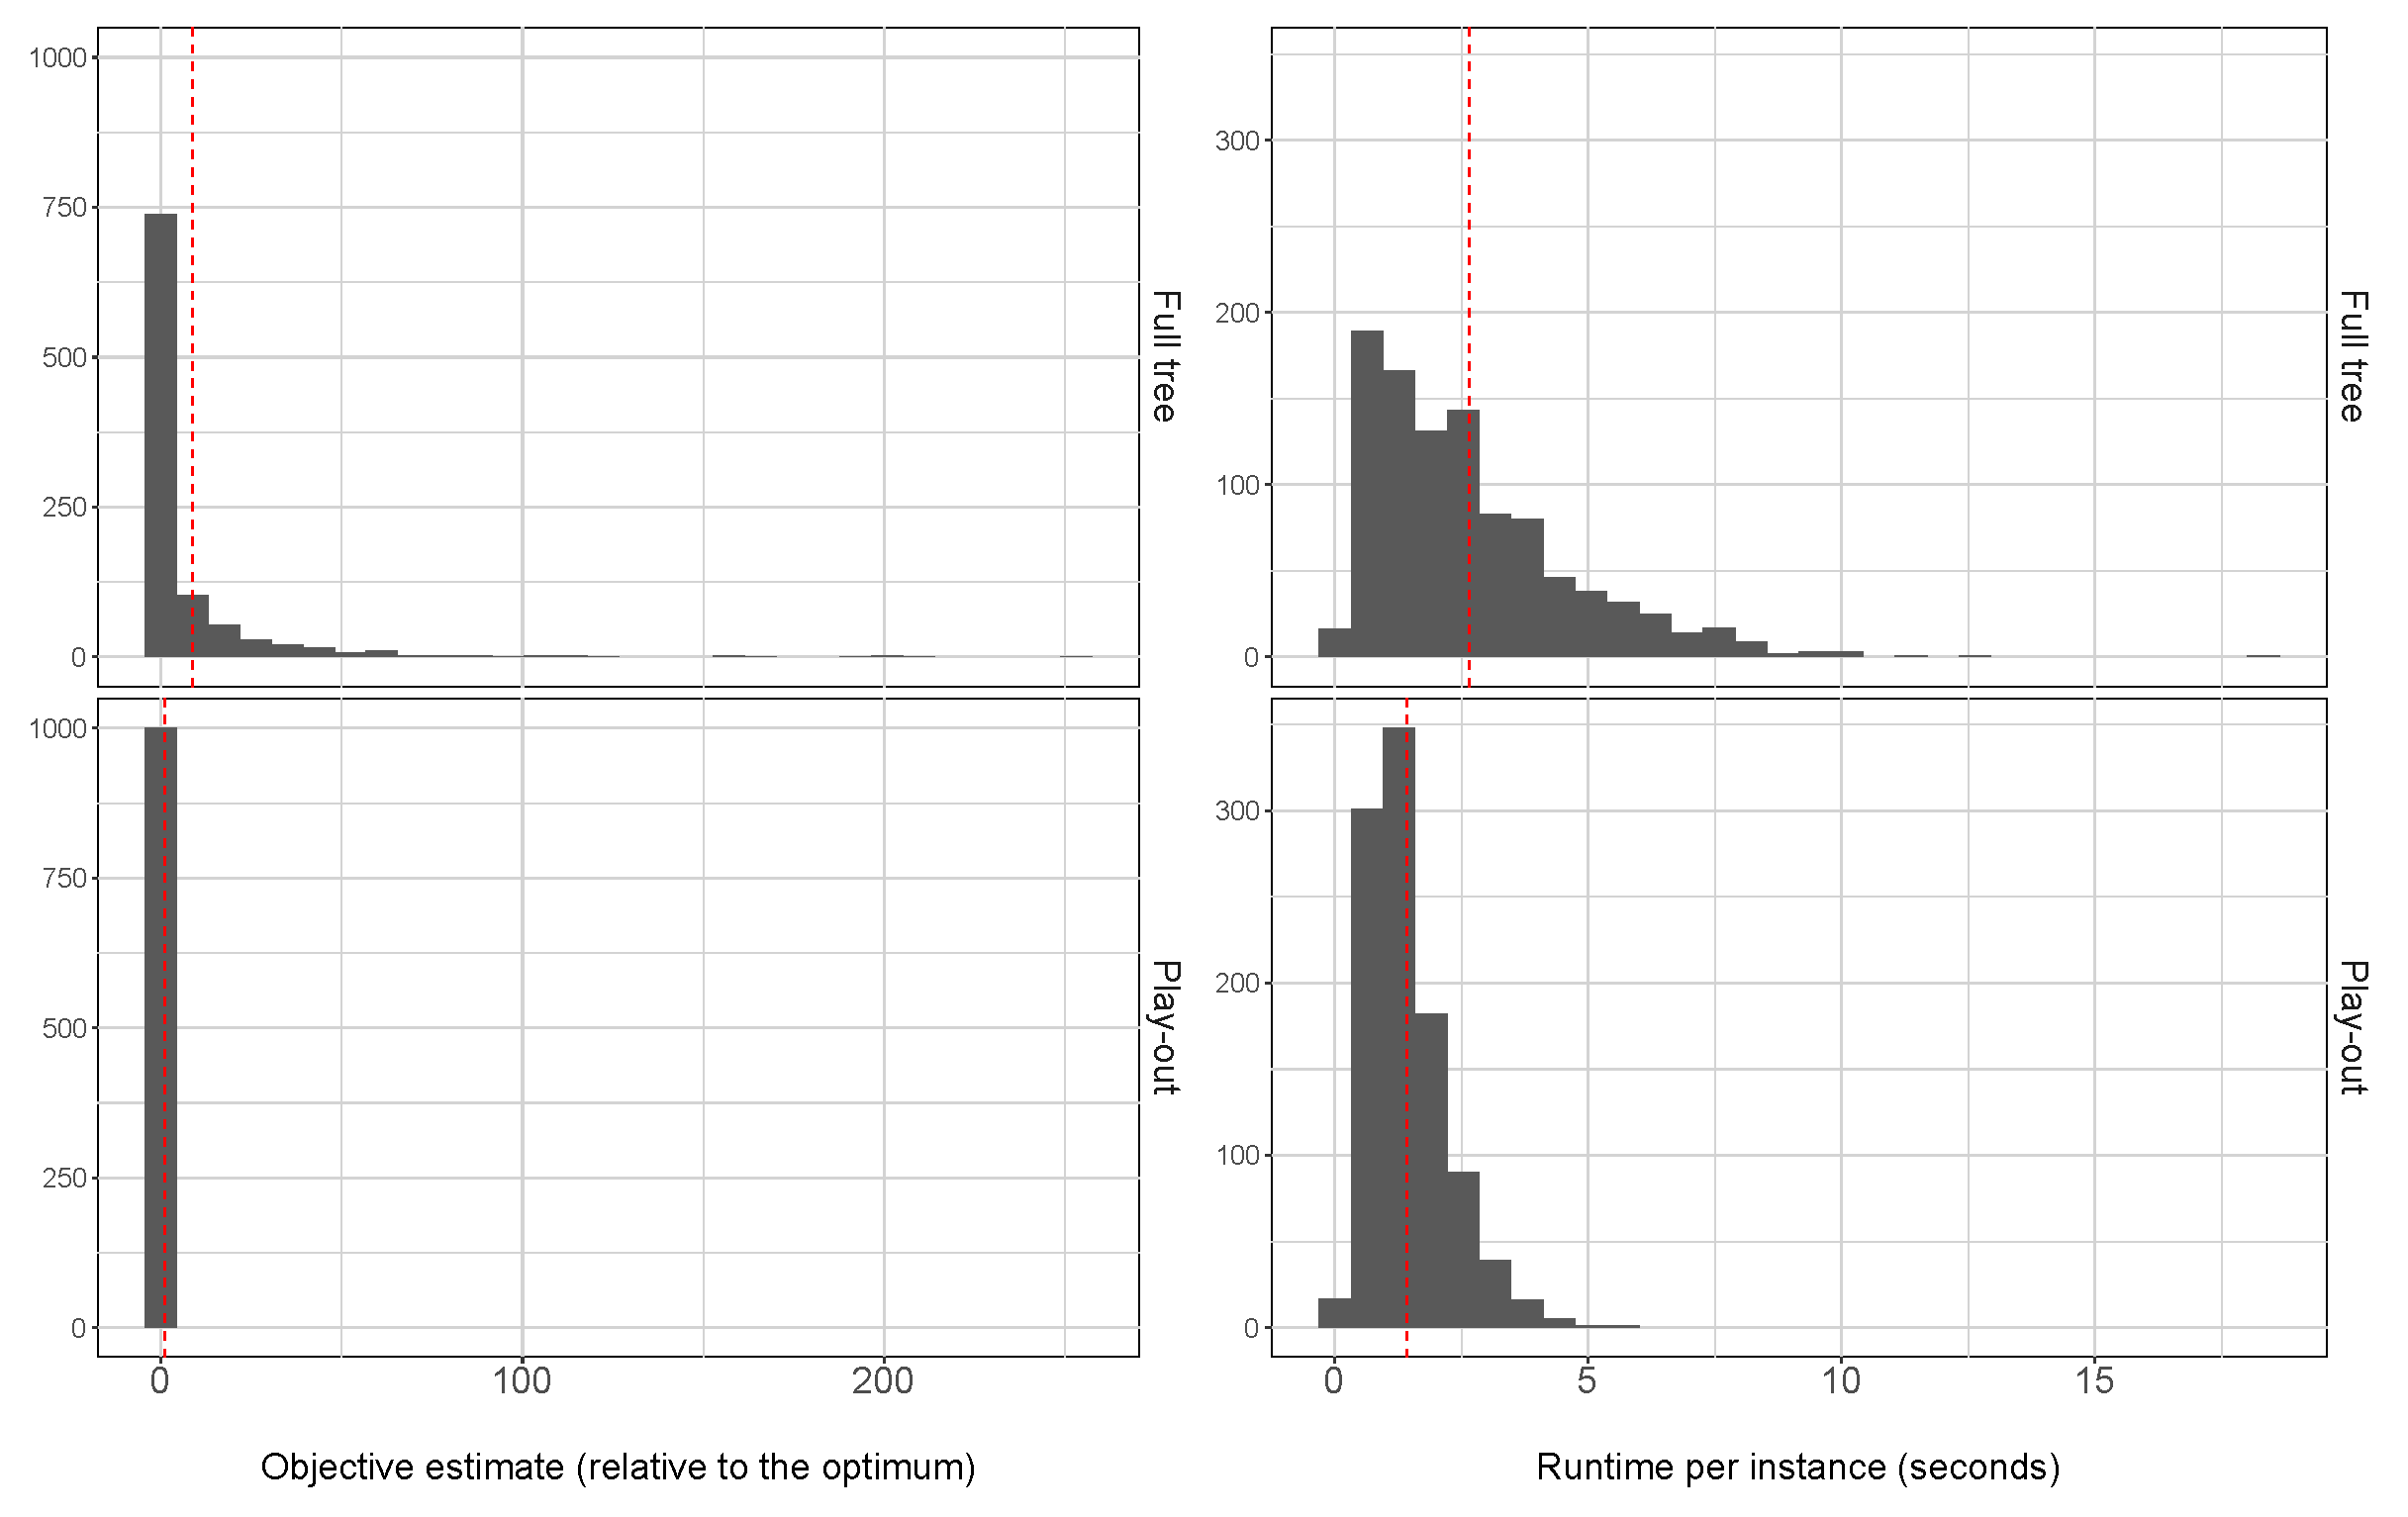
\includegraphics[width=\textwidth]{img/courage.eps}
\end{frame}
\subsection{On correctness}
\label{sec:org509e676}
\begin{frame}[label={sec:orgf068601}]{Why does it work? (A sketch on ``correctness'')}
\begin{theorem}[Proposition]
$$\lim_{k\rightarrow \infty} \mathbb{P}\{Q^k_{\rnode{}} = \textrm{true optimum}\}=1$$
\end{theorem}
A sketch of the proof:

\begin{itemize}
\item The game tree has finite number of nodes (there is a bound independent from \(K\)).
\item We never cut off all the optima \(\Rightarrow\) the tree contains at least one.
\item What is left is a finite-size minimax tree, containing an optimum.
\item As \(K\rightarrow\infty\), probability to select every node for expansion converges to 1.
\end{itemize}
\end{frame}

\begin{frame}[label={sec:org5c4df26}]{Why in the world the tree is finite?}
\begin{columns}
\begin{column}{0.15\columnwidth}
Network:
\centering
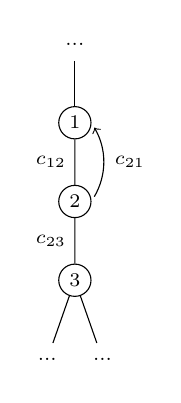
\begin{tikzpicture}[%level distance=5mm,
  level 1/.style={level distance=10mm,sibling distance=12mm},
  level 2/.style={level distance=10mm,sibling distance=7mm},
  level 3/.style={level distance=10mm,sibling distance=7mm},
  font=\scriptsize,inner sep=2pt,
  every node/.style={draw=black, circle}]
  \node[draw=none] {...}
  child {node (a) {1}
    child {node (b) {2}
      child {node (c) {3}
        child {node[draw=none] {...}}
        child {node[draw=none] {...}}
        edge from parent node[left, draw=none] {$c_{23}$}}
      edge from parent node[left, draw=none] {$c_{12}$}}};
  \draw[->, bend right, shorten >=2pt, shorten <=2pt] (b.east) to (a.east);
  \node[draw=none, fill=none, xshift=7mm] at ($(a)!.5!(b)$){$c_{21}$}; 
\end{tikzpicture}
\end{column}
\begin{column}{0.30\columnwidth}
After the \alert{first} expansion:
\vspace{2ex}

\centering
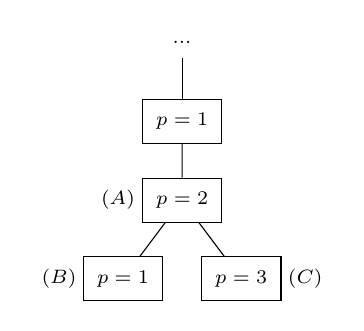
\begin{tikzpicture}[%level distance=5mm,
  level 1/.style={level distance=10mm,sibling distance=12mm},
  level 2/.style={level distance=10mm,sibling distance=7mm},
  level 3/.style={level distance=10mm,sibling distance=15mm},
  font=\scriptsize,inner sep=5pt,
  every node/.style={draw=black}]
  \node[draw=none] {...}
  child {node {$p=1$}
    child {node (A) {$p=2$}
      child {node (B) {$p=1$}}
      child {node (C) {$p=3$}}}};
  \node[draw=none, xshift=-3mm] at (A.west) {$(A)$};
  \node[draw=none, xshift=-3mm] at (B.west) {$(B)$};
  \node[draw=none, xshift=3mm] at (C.east) {$(C)$};
\end{tikzpicture}
\pause
\end{column}
\begin{column}{0.5\columnwidth}
After the \alert{second} expansion:
\vspace{2ex}

\centering
\begin{tikzpicture}[%level distance=5mm,
  level/.style={level distance=10mm,sibling distance=20mm},
  level 3/.style={sibling distance=30mm},
  font=\scriptsize,inner sep=5pt,
  every node/.style={draw=black}]
  \node[draw=none] {...}
  child {node {$p=1$}
    child {node (nA) {$p=2$}
      child {node[blue] (tn1) {$p=1$}
        child {node[blue] {$p=2$}
          child {node[blue] {$p=1$}
            child {node[draw=none] {...}}
            edge from parent[blue]}
          child {node[blue] (D) {$p=3$}
            child {node[draw=none] {...}}
            child {node[draw=none] {...}}
            edge from parent[blue]}
            edge from parent[blue]}
            edge from parent[blue]}
      child {node (nexit) {$p=3$}
        child {node[draw=none] {...}}
        child {node[draw=none] {...}}}}};
  \node[draw=none, xshift=3.5mm] at (nexit.east) {$(C)$};
  \node[draw=none, xshift=3.5mm] at (D.east) {$(D)$};
  \node[draw=none, xshift=-3mm] at (nA.west) {$(A)$};
  \node[draw=none, xshift=-3.5mm] at (tn1.west) {$(B)$};
\end{tikzpicture}
\end{column}
\end{columns}
\end{frame}
\section{{\bfseries\sffamily TODO} Conclusion}
\label{sec:orgf4ebbfc}
\subsection{Summary}
\label{sec:orgc513f47}
\subsection{Future research}
\label{sec:org83654f9}

\begin{frame}[label={sec:org3313e39}]{Mentioned sources}
 \scriptsize
\bibliographystyle{unsrtnat}
\bibliography{../../Dropbox/bibliography/references}
\end{frame}
\end{document}